\part{Oefeningen}
\chapter{Differentiaalvergelijkingen}
\exercise{Bepaal de DVG van \begin{enumerate}
                        \item $y = C_1x + C_2$
                        \item de cirkels met hun middelpunt op de x-as 
                        \item de raaklijnen aan $K: y = x^2$
                        \end{enumerate}}
{
\begin{enumerate}
\item De vergelijking $y = C_1x + C_2$ heeft 2 onafhankelijke constanten. Er moet dus 2 keer afgeleid worden.
\begin{equation*}
\begin{split}
y' & = C_1 \\
y'' & = 0
\end{split}
\end{equation*}
De differentiaalvergelijking is $y'' = 0$
\item Het middelpunt op de x-as kan gedefinieerd worden als $m \in x-as \Rightarrow m(C_1, 0)$. De straal wordt gedefinieerd als $C_2$. De vergelijking van een cirkel wordt dan:
$$\Gamma: (x - C_1)^2 + y^2 = C_2^2$$
Er zijn 2 onafhankelijke constanten. Er moet dus 2 keer (impliciet) afgeleid worden.
\begin{equation*}
\begin{split}
\frac{dy}{dx} :\; & 2(x - C_1) + 2yy' = 0 \\
\frac{d^2y}{dx^2} :\; & 2 + 2(y'y' + yy'') = 0
\end{split}
\end{equation*}
De 2de afgeleide bevat geen constanten meer dus de differentiaalvergelijking wordt: 
$$yy'' + (y')^2 + 1 = 0$$
\item De raaklijn wordt gegeven door : $R: y - y'p = y'_p(x - x_p)$

Stel $p \in K$ en $x_p = C$:
\begin{equation*}
\begin{split}
\Rightarrow & y_p = (x_p)^2 = C^2 \\
\Rightarrow & p(C, C^2)
\end{split}
\end{equation*}
De richtingscoëfficient $y'_p$ wordt gegeven door 
$$y'= 2x \Rightarrow y'_p = 2C$$

De formule van de raaklijn kan worden ingevuld:
$$R: (y - C^2) = 2C(x - C)$$
Deze vergelijking bevat slechts 1 constante en moet dus 1 maal afgeleid worden.
$$y' = 2C \Leftrightarrow C = \frac{y'}{2}$$
Substitueer $C$ in de formule van de raaklijn:
\begin{equation*}
\begin{split}
    & y - \bigg(\frac{y'}{2}\bigg)^2 = y'\bigg(\frac{y'}{2}\bigg)\bigg(x - \frac{y'}{2}\bigg) \\
    \Leftrightarrow \; & 4y - y'^2 = 4xy' - 2y'^2 \\
    \Leftrightarrow \; & y'^2 - 4y'x + 4y = 0
\end{split}
\end{equation*}
is de differentiaalvergelijking.
\end{enumerate}
}
\section{Lineaire DVG met constante coëfficiënten}
\exercise{
        Gegeven $$y'' + y = 0$$
        \begin{enumerate}
         \item Bepaal de AO
         \item Bepaal de PO zodat $y\big(\frac{\pi}{2}\big) = 0 $ en $y(\pi) = 1$
        \end{enumerate}

}{

}

\chapter{Laplacetransformatie}
\section{De Heaviside functie}
\begin{itemize}[label={}]
\item \exercise{Gegeven $$g(t) = \begin{cases}
                            0 & t < 0 \\
                            t &  0 < t < \frac{\pi}{2} \\
                            \sin t & \frac{\pi}{2} < t < \pi \\
                            0 & t > \pi         
                        \end{cases}
$$
Druk $g(t)$ uit a.d.h.v. de Heaviside functie en maak een tekening.}{
\begin{equation*}
\begin{split}
g(t) & = H(t)(-0 + t) + H(t - \frac{\pi}{2})(-t + \sin t) + H(t - \pi)(-\sin t + 0) \\
    & = H(t)t + H(t - \frac{\pi}{2})(\sin t - t) + H(t - \pi)(-\sin t) \\
    & = H(t)t + H(t - \frac{\pi}{2})(\sin t - t) - H(t - \pi)\sin t
\end{split}
\end{equation*}
\begin{center}
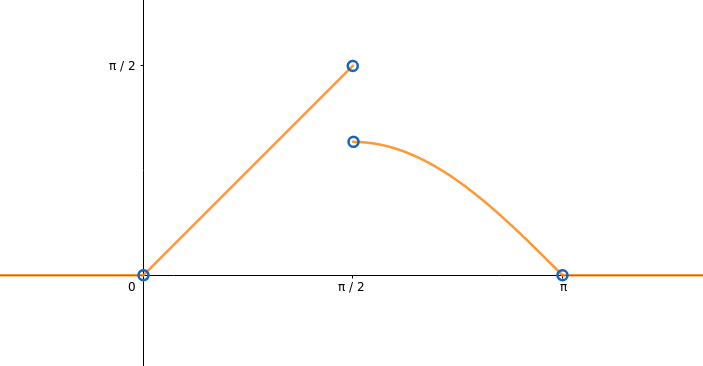
\includegraphics[width=0.9\textwidth]{oef2_heaviside}
\end{center}
}

\item{ \exercise{Gegeven de grafiek van de functie $h(t)$. Bepaal het voorschrift van $h(t)$ en druk uit a.d.h.v. de Heaviside functie.
\begin{center}
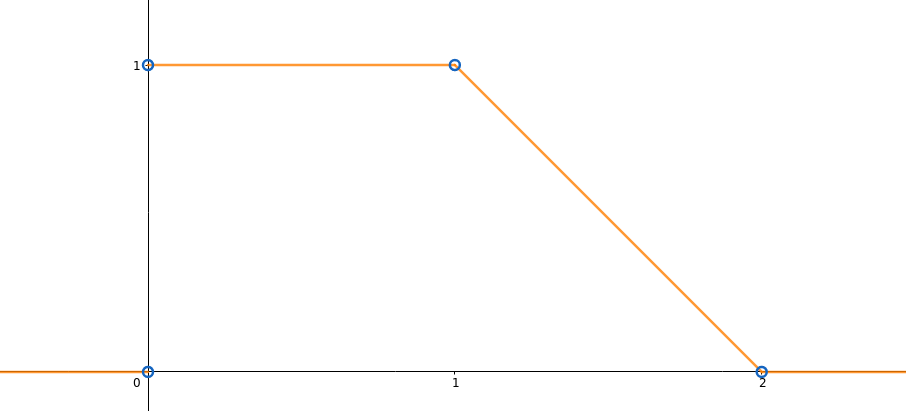
\includegraphics[width=0.9\textwidth]{oef3_heaviside}
\end{center}}{
De functie kan geschreven worden als:
$$h(t) = \begin{cases}
        0 & t < 0 \\
        1 & 0 < t < 1 \\
        2 - t & 1 < t < 2 \\
        0 & t > 2
        \end{cases}
$$
Hieruit volgt gemakkelijk de Heaviside versie hiervan:
\begin{equation*}
\begin{split}
h(t) & = H(t)(-0 + 1) + H(t - 1)(-1 + (2 - t)) + H(t-2)(-(2-t) + 0) \\
    & = H(t) + H(t-1)(1 - t) + H(t- 2)(t - 2)
\end{split}
\end{equation*}}}
\item{
    \exercise{
        Teken de functie $f(t) = 1 + H(t-1)(e^{t}-1) + H(t-2)(2-e^{t})$
    }{
        $$f(t) = \begin{cases}
                    1   & t < 1     \\
                    e^t & 0 < t < 1 \\
                    2   & 1 < t < 2
                 \end{cases}
        $$
        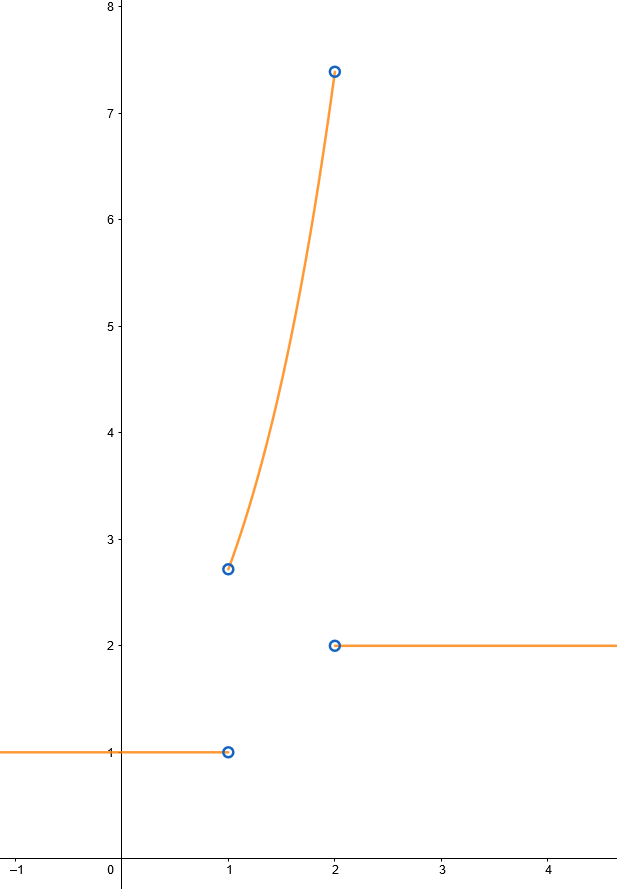
\includegraphics[width=0.9\textwidth]{oef4_heaviside}
    }
}
\end{itemize}
\section{Functies van de exponentiële orde}
\begin{itemize}[label={}]
 \item{
    \exercise{
            Geef de exponentiële orde van $f(t) = te^{-2t}$
    }{
            \begin{equation*}
             \begin{split}
              \lim_{t \to +\infty} \frac{|te^{-2t}|}{e^{\alpha t}} & = \lim_{t \to +\infty} \frac{te^{-2t}}{e^{\alpha t}} \\
                                                                   & = \lim_{t \to +\infty} \frac{t}{e^{\alpha t}e^{2t}}  \\
                                                                   & = \lim_{t \to +\infty} \frac{t}{e^{t(\alpha + 2)}}   \\
                                                                   & \stackrel{H}{=} \lim_{t \to +\infty} \frac{1}{e^{t(\alpha + 2)}(\alpha + 2)} \qquad \hbox{voor}\; \alpha + 2 > 0 \\
                                                                   & = 0 \in \mathbb{R}
             \end{split}
            \end{equation*}
            Dus
            \begin{equation*}
             \begin{split}
                              & \alpha + 2 > 0 \\
              \Leftrightarrow & \alpha > -2
             \end{split}
            \end{equation*}
            De exponentiële orde is -2.
        }}
 \item{
    \exercise{
        Geef de exponentiële orde van $f(t) = 6e^{3t}$
    }{
        \begin{equation*}
         \begin{split}
          \lim_{t \to +\infty} \frac{|6e^{3t}|}{e^{\alpha t}} & = \lim_{t \to +\infty} \frac{6e^{3t}}{e^{\alpha t}} \\
                                                              & = 6\lim_{t \to +\infty} e^{t(3 - \alpha)} \\                                                    
         \end{split}
        \end{equation*}
        Indien $ 3 - \alpha < 0$ dan wordt de limiet 0. De exponentiële orde is dus 3.
    }
 
 }
\end{itemize}
\section{Laplacebeeld}
Bepaal het Laplacebeeld van volgende functies:
\begin{itemize}[label={}]
 \item{
    \exercise{
        $f(t) = 3e^{2t} + t^2 - 5\cos 2t + 4\sin 3t$
    }{
        \begin{equation*}
         \begin{split}
          \mathcal{L}\{3e^{2t} + t^2 - 5\cos 2t + 4\sin 3t\}(s) = \frac{3}{s - 2} + \frac{2}{s^3} - \frac{5s}{s^2 + 4} + \frac{12}{s^2 + 9}
         \end{split}
        \end{equation*}
    }
 }
 \item{
    \exercise{
        $f(t) = (1 + e^{-4t})^2$
    }{
        \begin{equation*}
         \begin{split}
          \mathcal{L}\{(1 + e^{-4t})^2\}(s) & = \mathcal{L}\{1 + 2e^{-4t} + e^{-8t}\}(s) \\
                                            & = \frac{1}{s} + \frac{2}{s + 4} + \frac{1}{s + 8}
         \end{split}
        \end{equation*}
    }
 }
 \item{
    \exercise{
        $f(t) = \sin^2 t$
    }{
        \begin{equation*}
         \begin{split}
          \mathcal{L}\{\sin^2 t\}(s) & = \mathcal{L}\{\frac{1 - \cos 2t}{2}\}(s) \\
                                     & = \frac{1}{2}\mathcal{L}\{1 - \cos 2t\} \\
                                     & = \frac{1}{2}\bigg[\frac{1}{s} - \frac{s}{s^2 + 4}\bigg]
         \end{split}
        \end{equation*}
    }
 }
 \item{
    \exercise{
        $f(t) = t^2\delta(t - 2)$
    }{
        \begin{equation*}
         \begin{split}
          \mathcal{L}\{t^2\delta(t - 2)\}(s) & = \int_{0}^{+\infty} t^2\delta(t-2)e^{-st}\;dt \\
                                             & = [t^2e^{-st}]_{t = 2} \\
                                             & = 4e^{-2s}
         \end{split}
        \end{equation*}
    }
 }
 \item{
    \exercise{
        $f(t) = (t - 1)H(t - 1)$
    }{
        \begin{equation*}
         \begin{split}
          \mathcal{L}\{(t - 1)H(t - 1\}(s) & = e^{-s}\mathcal{L}\{u\}(s) \\
                                           & = \frac{e^{-s}}{s^2}
         \end{split}
        \end{equation*}
    }
 }
 \item{
    \exercise{
        $f(t) = t^2H(t-1)$
    }{
        \begin{equation*}
         \begin{split}
          \mathcal{L}\{t^2H(t-1)\}(s) & = \mathcal{L}\{[(t-1)+1]^2H(t-1)\}(s) \\
                                      & = \mathcal{L}\{(t-1)^2 + 2(t-1)+1)H(t-1)\}(s) \\
                                      & = e^{-s}\mathcal{L}\{u^2 + 2u + 1\} \\
                                      & = e^{-s}\bigg(\frac{2}{s^3} + \frac{2}{s} + \frac{1}{s}\bigg)
         \end{split}
        \end{equation*}
    }
 }
 \item{
    \exercise{
        $f(t) = t^2H(t-1)$
    }{
        \begin{equation*}
         \begin{split}
          \mathcal{L}\{t^2H(t-1)\}(s) & = \mathcal{L}\{[(t-1)+1]^2H(t-1)\}(s) \\
                                      & = \mathcal{L}\{(t-1)^2 + 2(t-1)+1)H(t-1)\}(s) \\
                                      & = e^{-s}\mathcal{L}\{u^2 + 2u + 1\} \\
                                      & = e^{-s}\bigg(\frac{2}{s^3} + \frac{2}{s} + \frac{1}{s}\bigg)
         \end{split}
        \end{equation*}
    }
 }
 \item{
    \exercise{
        $f(t) = \sin(t)H(t-2)$
    }{
        \begin{equation*}
         \begin{split}
          \mathcal{L}\{\sin(t)H(t-2)\}(s) & = \mathcal{L}\{\sin((t - 2) + 2)H(t-2)\}(s) \\
                                          & = \mathcal{L}\{[\sin(t-2)\cos(2) + \cos(t-2)\sin(2)]H(t-2)\}(s) \\
                                          & = \mathcal{L}\{[\sin(t-2)\cos(2) + \cos(t-2)\sin(2)]H(t-2)\}(s) \\
                                          & = e^{-2s}[\cos(2)\mathcal{L}\{\sin(u)\} + \sin(2)\mathcal{L}\{\cos(u)\}(s)] \\
                                          & = e^{-2s}\bigg(\frac{\cos(2)}{s^2+1} + \frac{\sin(2)s}{s^2 + 1}\bigg)
         \end{split}
        \end{equation*}
    }
 }
 \item{
    \exercise{
        $f(t) = t^2e^{-2t}$
    }{
        \begin{equation*}
         \begin{split}
          \mathcal{L}\{t^2e^{-2t}\}(s) & = \mathcal{L}\{t^2\}(s + 2) \\
                                       & = \frac{2}{(s+2)^3}
         \end{split}
        \end{equation*}
    }
 }
 \item{
    \exercise{
        $f(t) = e^t\cos 3t$
    }{
        \begin{equation*}
         \begin{split}
          \mathcal{L}\{e^t\cos 3t\}(s) & = \mathcal{L}\{\cos 3t\}(s - 1) \\
                                       & = \frac{s - 1}{(s - 1)^2 + 9} 
         \end{split}
        \end{equation*}
    }
 }
 \item{
    \exercise{
        $f(t) = e^{-2t}\sin 2t$
    }{
        \begin{equation*}
         \begin{split}
          \mathcal{L}\{e^{-2t}\sin 2t\}(s) & = \mathcal{L}\{\sin 2t\}(s + 2) \\
                                       & = \frac{2}{(s + 2)^2 + 4}
         \end{split}
        \end{equation*}
    }
 }
 \item{
    \exercise{
        $f(t) = t\cos t$
    }{
        \begin{equation*}
         \begin{split}
          \mathcal{L}\{t\cos t\}(s) & = (-1)^1 \frac{d\bigg[\mathcal{L}\{\cos t\}(s)\bigg]}{ds} \\
                                    & = - \frac{d[\frac{s}{s^2 + 1}]}{ds} \\
                                    & = -\frac{(s^2 + 1) - s(2s)}{(s^2 + 1)^2} \\
                                    & = -\frac{s^2 + 1 - 2s^2}{(s^2 + 1)^2} \\
                                    & = \frac{s^2 - 1}{(s^2 + 1)^2}
         \end{split}
        \end{equation*}
    }
 }
 
 \item{
    \exercise{
        $f(t) = e^{-2t}t\cos^2 \frac{t}{2}$
    }{
        \begin{equation*}
         \begin{split}
          \mathcal{L}\{e^{-2t}t\cos^2 \frac{t}{2}\}(s) & = \mathcal{L}\{t\cos^2 \frac{t}{2}\}(s + 2) \\
                                                       & = \mathcal{L}\bigg\{t\frac{1 + \cos t}{2}\bigg\}(s + 2) \\
                                                       & = \frac{1}{2}\bigg(\mathcal{L}\{t\}(s + 2) + \mathcal{L}\{t \cos t\}(s+2)\bigg) \\
                                                       & = \frac{1}{2}\bigg(\frac{1}{(s+2)^2} + \frac{(s+2)^2 - 1}{((s+2)^2 + 1)^2}\bigg) \\
         \end{split}
        \end{equation*}
    }
 }
 \item{
    \exercise{
        $f(t) = e^{-3t}t^3H(t - 2)$
    }{
        \begin{equation*}
         \begin{split}
          \mathcal{L}\{e^{-3t}t^3H(t - 2)\}(s) & = \mathcal{L}\{t^3H(t - 2)\}(s + 3) \\
                                               & = \mathcal{L}\{[(t-2)+2]^3H(t-2)\}(s + 3) \\
                                               & = \mathcal{L}\{[(t-2)^3 + 6(t-2)^2+12(t-2) + 8]H(t-2)\}(s + 3) \\
                                               & = e^{2s}\mathcal{L}\{u^3 + 6u^2 + 12u + 8\}(s + 3) \\
                                               & = e^{2s}\bigg[\frac{3!}{(s+3)^4}+6\frac{2!}{(s+3)^3}+12\frac{1!}{(s+3)^2} + 8\frac{1}{s}\bigg] \\
                                               & = e^{2s}\bigg[\frac{6}{(s+3)^4}+\frac{12}{(s+3)^3}+\frac{12}{(s+3)^2} + \frac{8}{s}\bigg] \\
                                               & = 2e^{2s}\bigg[\frac{3}{(s+3)^4}+\frac{6}{(s+3)^3}+\frac{6}{(s+3)^2} + \frac{4}{s}\bigg]
         \end{split}
        \end{equation*}
    }
 }
 \item{
    \exercise{
        $f(t) = \begin{cases}
                 \cos 2t & 0 < t < \frac{\pi}{4} \\
                 e^{2t}t & t > \frac{\pi}{4}
                \end{cases}$

    }{
        \begin{equation*}
         \begin{split}
          f(t) & = \cos 2t + H\big(t-\frac{\pi}{4}\big)(-\cos 2t + e^{2t}t) \\
               & = \cos 2t + (e^{2t}t - \cos 2t)H\big(t - \frac{\pi}{4}\big) \\
          \mathcal{L}\{f(t)\}(s) & = \mathcal{L}\{\cos 2t\}(s) + \mathcal{L}\{e^{2t}tH\big(t - \frac{\pi}{4}\big)\}(s) - \mathcal{L}\{\cos(2t)H\big(t - \frac{\pi}{4}\big)\}(s)
         \end{split}
        \end{equation*}
    We lossen deze 3 Laplacetransformaties individueel op
    \begin{enumerate}
     \item \begin{equation*}
            \begin{split}
                \mathcal{L}\{\cos 2t\}(s) = \frac{s}{s^2 + 4}
            \end{split}
           \end{equation*}
     \item \begin{equation*}
            \begin{split}
                    \mathcal{L}\{e^{2t}tH\big(t - \frac{\pi}{4}\big)\}(s) & = \mathcal{L}\{tH\big(t - \frac{\pi}{4}\big)\}(s - 2) \\
                                                                        & = \mathcal{L}\{\big(t - \frac{\pi}{4} + \frac{\pi}{4}\big)H\big(t - \frac{\pi}{4}\big)\}(s - 2) \\
                                                                        & = e^{-\frac{\pi}{4}s}\mathcal{L}\{\big(u + \frac{\pi}{4}\big)\}(s - 2) \\
                                                                        & = e^{-\frac{\pi}{4}s}\bigg(\frac{1}{(s - 2)^2} +  \frac{\pi}{4(s - 2)}\bigg)
              \end{split}
             \end{equation*}
    \item \begin{equation*}
            \begin{split}
                \mathcal{L}\{\cos 2t\;H\big(t - \frac{\pi}{4}\big)\}(s) & = \mathcal{L}\{\cos \big[2\big(t-\frac{\pi}{4} + \frac{\pi}{4}\big)\big]H\big(t - \frac{\pi}{4}\big)\}(s) \\
                                                                        & = \mathcal{L}\{\cos\big[2\big(t - \frac{\pi}{4}\big) + \frac{\pi}{2}\big]H\big(t - \frac{\pi}{4}\big)\}(s) \\
                                                                        & = \mathcal{L}\{[\cos 2(t - \frac{\pi}{4})\cos\frac{\pi}{2} - \sin 2(t - \frac{\pi}{4})\sin\frac{\pi}{2}]H\big(t - \frac{\pi}{4})\}(s) \\
                                                                        & = - \mathcal{L}\{\sin 2(t - \frac{\pi}{4})H(t - \frac{\pi}{4}\}(s) \\
                                                                        & = e^{-\frac{\pi}{4}s}\mathcal{L}\{\sin 2u\} \\
                                                                        & = \frac{2e^{-\frac{\pi}{4}s}}{s^2 + 4}
            \end{split}
           \end{equation*}
    \end{enumerate}
    Uiteindelijk:
    $$\mathcal{L}\{f(t)\}(s) = \frac{s}{s^2 + 4} + e^{-\frac{\pi}{4}s}\bigg(\frac{1}{(s - 2)^2} +  \frac{\pi}{4(s - 2)}\bigg) - \frac{2e^{-\frac{\pi}{4}s}}{s^2 + 4}$$
    }
 }
 
 
\end{itemize}

\section{Invers Laplacebeeld}
Bepaal het invers laplacebeeld van volgende functies:
\begin{itemize}[label={}]
 \item{
    \exercise{
        $$f(s) = \frac{1}{s^3}$$
    }{
        \begin{equation*}
         \begin{split}
          \mathcal{L}^{-1}\bigg\{\frac{1}{s^3}\bigg\}(t) & = \frac{1}{2!}\mathcal{L}^{-1}\bigg\{\frac{2!}{s^3}\bigg\}(t) \\
                                                         & = \frac{t^2}{2}
         \end{split}
        \end{equation*}
    }
 }
 \item{
    \exercise{
        $$f(s) = \frac{s + 5}{s^4}$$
    }{
        \begin{equation*}
         \begin{split}
          \mathcal{L}^{-1}\bigg\{\frac{s + 5}{s^4}\bigg\}(t) & = \mathcal{L}^{-1}\bigg\{\frac{s}{s^4} + \frac{5}{s^4}\bigg\}(t) \\
                                                             & = \mathcal{L}^{-1}\bigg\{\frac{1}{s^3}\bigg\}(t) + 5\mathcal{L}^{-1}\bigg\{\frac{5}{s^4}\bigg\}(t) \\
                                                             & = \frac{1}{2!}\mathcal{L}^{-1}\bigg\{\frac{2!}{s^3}\bigg\}(t) + \frac{5}{3!}\mathcal{L}^{-1}\bigg\{\frac{3!}{s^4}\bigg\}(t) \\
                                                             & = \frac{t^2}{2} + \frac{5t^3}{6}
         \end{split}
        \end{equation*}
    }
 }
 \item{
    \exercise{
        $$f(s) = \frac{1}{3s - 1}$$
    }{
        \begin{equation*}
         \begin{split}
          \mathcal{L}^{-1}\bigg\{\frac{1}{3s - 1}\bigg\}(t) & = \frac{1}{3}\mathcal{L}^{-1}\bigg\{\frac{1}{s - \frac{1}{3}}\bigg\}(t) \\
                                                            & = \frac{1}{3}e^{\frac{1}{3}t} \\
                                                            & = \frac{1}{3}e^{\frac{t}{3}}
         \end{split}
        \end{equation*}
    }
 }
 \item{
    \exercise{
        $$f(s) = \frac{2s + 3}{s^2 - 5s + 6}$$
    }{
        \begin{equation*}
         \begin{split}
          \mathcal{L}^{-1}\bigg\{\frac{2s + 3}{s^2 - 5s + 6}\bigg\}(t) & = \mathcal{L}^{-1}\bigg\{\frac{2s + 3}{(s-2)(s-3)}\bigg\}(t) \\
          \Rightarrow & \frac{2s + 3}{(s-2)(s-3)} = \frac{a}{s - 2} + \frac{b}{s-3} = \frac{a(s-3) + b(s-2)}{(s-2)(s-3)} \\
          \Rightarrow & 2s + 3 = a(s-3) + b(s-2) \Rightarrow \begin{cases}
                                                              a = -7 \\
                                                              b = 9
                                                             \end{cases} \\
                                                             & =  \mathcal{L}^{-1}\bigg\{\frac{-7}{s - 2} + \frac{9}{s - 3}\bigg\}(t) \\
                                                             & = -7e^{2t} + 9e^{3t}
         \end{split}
        \end{equation*}
    }
 }
 \item{
    \exercise{
        $$f(s) = \frac{4s + 3}{s^2 + 16}$$
    }{
        \begin{equation*}
         \begin{split}
          \mathcal{L}^{-1}\bigg\{\frac{4s + 3}{s^2 + 16}\bigg\}(t) & = \mathcal{L}^{-1}\bigg\{\frac{4s}{s^2 + 16} + \frac{3}{s^2 + 16}\bigg\}(t) \\
          & = 4\cos 4t + \frac{3}{4}\sin 4t
         \end{split}
        \end{equation*}
    }
 }
 \item{
    \exercise{
        $$f(s) = \frac{s + 3}{s(s^2 + 9)}$$
    }{
        \begin{equation*}
         \begin{split}
          \mathcal{L}^{-1}\bigg\{\frac{s + 3}{s(s^2 + 9)}\bigg\}(t) \\
          \Rightarrow & \frac{s + 3}{s(s^2 + 9)} = \frac{a}{s} + \frac{b + cs}{s^2 + 9} = \frac{a(s^2 + 9) + (b+cs)s}{s(s^2 + 9)} \\
          \Rightarrow & s + 3 = a(s^2 + 9) + (b + cs)s \Rightarrow \begin{cases}
                                                                    a = \frac{1}{3} \\
                                                                    b = -\frac{1}{3} \\
                                                                    c = 1
                                                                   \end{cases} \\
                    & = \mathcal{L}^{-1}\bigg\{\frac{1}{3s} \bigg\} + \mathcal{L}^{-1}\bigg\{\frac{-\frac{1}{3}}{s^2 + 9} \bigg\} + \mathcal{L}^{-1}\bigg\{\frac{s}{s^2 + 9} \bigg\} \\
                    & = \frac{1}{3} - \frac{1}{3}\cdot\frac{1}{3}\mathcal{L}^{-1}\bigg\{\frac{3}{s^2 + 9}\bigg\} + \cos 3t \\
                    & = \frac{1}{3} - \frac{1}{9}\sin 3t + \cos 3t
         \end{split}
        \end{equation*}
    }
 }
 \item{
    \exercise{
        $$f(s) = \frac{1}{s + 3}^2$$
    }{
       \begin{equation*}
        \begin{split}
            \bigginvlaplace{\frac{1}{s + 3}^2} & = e^{-3t}\bigginvlaplace{\frac{1}{s^2}} \\
                                               & = te^{-3t}
        \end{split}
       \end{equation*}

    }
 }
 \item{
    \exercise{
        $$f(s) = \frac{2s + 5}{(s + 2)^3}$$
    }{
       \begin{equation*}
        \begin{split}
            \bigginvlaplace{\frac{2s + 5}{(s + 2)^3}} & = \bigginvlaplace{\frac{2[(s + 2) - 2] + 5}{(s + 2)^3}} \\
                                                      & = 2\bigginvlaplace{\frac{1}{(s+2)^2}} + \bigginvlaplace{\frac{1}{(s + 2)^3}} \\
                                                      & = 2e^{-2t}\bigginvlaplace{\frac{1}{s^2}} + \frac{e^{2t}}{2!}\bigginvlaplace{\frac{2!}{s^3}} \\
                                                      & = e^{2t}\big(2t + \frac{1}{2}t^2\big)
        \end{split}
       \end{equation*}

    }
 }
 \item{
    \exercise{
        $$f(s) = \frac{2s - 3}{s^2 + 2s + 5}$$
    }{
       \begin{equation*}
        \begin{split}
            \bigginvlaplace{\frac{2s - 3}{s^2 + 2s + 5}} & = \bigginvlaplace{\frac{2(s + 1) + 1}{(s + 1)^2 + 4}} \\
                                                         & = 2\bigginvlaplace{\frac{s + 1}{(s + 1)^2 + 4}} + \bigginvlaplace{\frac{1}{(s + 1)^2 + 4}} \\
                                                         & = 2e^{-t}\bigginvlaplace{\frac{s}{s^2 + 4}} + \frac{e^{-t}}{2}\bigginvlaplace{\frac{2}{s^2 + 4}} \\
                                                         e^{-t}\bigg(2\cos 2t + \frac{1}{2}\sin 2t\bigg)
        \end{split}
       \end{equation*}

    }
 }
 \item{
    \exercise{
        $$f(s) = \frac{e^{-s}}{s^4}$$
    }{
       \begin{equation*}
        \begin{split}
            \bigginvlaplace{\frac{e^{-s}}{s^4}} & = f(t - 1)H(t - 1) \\
                \hbox{met} & f(t) = \bigginvlaplace{\frac{1}{s^4}} = \frac{t^3}{6} \\
            \Rightarrow & \frac{(t - 1)^3}{6}H(t - 1)
        \end{split}
       \end{equation*}

    }
 }
 \item{
    \exercise{
        $$f(s) = \frac{e^{-3s}}{s + 2}$$
    }{
       \begin{equation*}
        \begin{split}
            \bigginvlaplace{\frac{e^{-3s}}{s + 2}} & = f(t - 3)H(t - 3) \\
                \hbox{met} & f(t) = \bigginvlaplace{\frac{1}{ s + 2 }} = e^{-2t} \\
            \Rightarrow & e^{-2(t - 3)}H(t - 3)
        \end{split}
       \end{equation*}

    }
 }
 \item{
    \exercise{
        $$f(s) = \frac{e^{-2s}}{(s + 3)^5}$$
    }{
       \begin{equation*}
        \begin{split}
            \bigginvlaplace{\frac{e^{-2s}}{(s + 3)^5}} & = f(t - 2)H(t - 2) \\
                \hbox{met} & f(t) = \bigginvlaplace{\frac{1}{(s+3)^5}} = e^{-3t}\bigginvlaplace{\frac{1}{s^5}} = \frac{e^{-3t}}{4!}t^4 \\
            \Rightarrow & \frac{e^{-3(t-2)}(t - 2)^4}{4!}H(t - 2)
        \end{split}
       \end{equation*}

    }
 }
 \item{
    \exercise{
        $$f(s) = \frac{3s^3 - 4s^2 + 1}{s^2(s^2 - 2s + 2)}$$
    }{
       \begin{equation*}
        \begin{split}
            \bigginvlaplace{\frac{3s^3 - 4s^2 + 1}{s^2(s^2 - 2s + 2)}} & = \hbox{splitsen in partieël breuken} \\  
            & = \frac{1}{2}\bigginvlaplace{\frac{1}{s}} +  \frac{1}{2}\bigginvlaplace{\frac{1}{s^2}} +  \frac{1}{2}\bigginvlaplace{\frac{5s - 7}{s^2 - 2s + 2}} \\
            & = \frac{1}{2}\bigg[1 + t + \bigginvlaplace{\frac{5(s - 1) - 2}{(s - 1)^2 + 1}} \bigg] \\
            & = \frac{1}{2}\bigg[1 + t + 5e^t\cos t - 2e^t\sin t\bigg]
        \end{split}
       \end{equation*}

    }
 }
 \item{
    \exercise{
        $$f(s) = \frac{s}{(s^2 + 4)^2}$$
    }{
       \begin{equation*}
        \begin{split}
            \bigginvlaplace{\frac{s}{(s^2 + 4)^2}} & = -\frac{1}{4}\bigginvlaplace{\frac{d}{ds}\bigg(\frac{2}{s^2 + 4}\bigg)} \\
                                                   & = -\frac{1}{4}(-1)t\sin 2t \\
                                                   & = \frac{t}{4}\sin 2t
        \end{split}
       \end{equation*}

    }
 }
 \item{
    \exercise{
        Bepaal het inverselaplacebeeld met convolutie van $$f(s) = \frac{1}{s^2 - 1}$$
    }{
       \begin{equation*}
        \begin{split}
            \bigginvlaplace{\frac{1}{s^2 - 1}} & = \bigginvlaplace{\frac{1}{s + 1}\cdot \frac{1}{s - 1}} \\
                                               & = e^t * e^{-t} \\
                                               & = \int_0^t e^{u}e^{-(t - u)}\; du \\
                                               & = \int_0^t e^{2u -t }\; du\\
                                               & = \bigg[\frac{1}{2}e^{2u - t} \bigg]_{u = 0}^{u = t} \\
                                               & = \frac{1}{2}\big[e^{t}-e^{-t}\big]
        \end{split}
       \end{equation*}

    }
 }
\end{itemize}




\end{document}

